\documentclass[pdflatex,iicol,sn-mathphys-num]{sn-jnl}
\usepackage{graphicx,amsmath,amssymb,booktabs}
\raggedbottom
\newcommand{\qmom}{\bar{\gamma}_{\rm mom}}
\newcommand{\gproxy}{\gamma_{\rm sel}}
\newcommand{\eb}{e\,{\rm b}}
\begin{document}

\title[Quadrupole diagnostics in odd Ba]{Spin-channel redistribution in quadrupole shape diagnostics of odd barium}
\author{\fnm{Author information} \sur{pending}}
\affil{\orgname{Research draft; author and affiliation details to be supplied}}

\abstract{Convergence of a quadrupole diagnostic within one intermediate-spin channel does not establish how its evolution relates to intrinsic charge shape. An unpaired particle--rotor control isolates this question by fixing the charge tensor at $\gamma=20^\circ$: complete moments remain constant while the fully summed selected-channel ratio changes and leaves the real-angle domain. We then resolve the coupling response in the lowest $11/2^-$ states of $^{129-137}$Ba within an explicitly specified interacting boson--fermion model. Five states exhaust more than $99.5\%$ of the selected-channel quadratic strength but only $20.0$--$28.9\%$ of the complete moment. A fixed-operator intervention identifies the redistribution of static strength and signed cubic paths behind their different responses. Alternative charge calibrations and a failed conditional high-spin isomer check limit the empirical interpretation of the Ba calculation. The fixed-geometry counterexample and the finite-model mechanism together show why angular-channel coverage and coupling response must be assessed separately from state-count convergence when converting a selected diagnostic into a shape coordinate.}
\keywords{quadrupole invariants, odd-mass nuclei, interacting boson--fermion model, barium isotopes}
\maketitle

\section{Introduction}\label{sec:intro}

Electric-quadrupole matrix elements connect nuclear spectroscopy to collective shape. Their scalar products describe charge distributions without choosing a laboratory orientation, and their relation to deformation has long been developed in the quadrupole-invariant formalism \cite{Cline1986}. In practice, only a restricted matrix-element network may be available. The quality of a deformation estimate then depends on which matrix elements are retained as well as how accurately they are known. Approximations using a few observables and the convergence of finite sums have been examined in rotor, interacting-boson and shell-model calculations \cite{Werner2005,Henderson2020}.

This distinction is particularly relevant to odd nuclei. A rank-two tensor acting on a state with spin $J$ connects several intermediate spins, and particle--core coupling can redistribute strength among them. Nomura and collaborators already showed that indicators based on different $\Delta J$ selections can evolve differently in odd-mass Eu and Sm \cite{Nomura2016}. For the $\gamma$-soft region near $A=130$, their interacting boson--fermion model (IBFM) study used effective quadrupole coordinates constructed from the lowest five $J+2$ states \cite{Nomura2017}. Such a selection defines legitimate rotational scalars. Its convergence, however, does not establish equivalence to the complete charge-polynomial moments.

We test this inference with a rigid-charge particle--rotor control that holds the intrinsic tensor exactly fixed while varying angular coupling. A separate odd-Ba IBFM calculation then compares complete and restricted quantities on the same states, at fixed initial spin and with the same electric-quadrupole operator. Its controlled coupling path resolves the redistribution of static strength and signed cubic contributions. Electromagnetic constraints delimit the application of this mechanism to the actual nuclei. The Ba study uses published Hamiltonian parameters but does not reproduce or correct the published electromagnetic-invariant figures.

\section{Model and quadrupole diagnostics}\label{sec:method}

\subsection{Fixed Hamiltonians and calibrated charge operator}

We couple one $h_{11/2}$ neutron quasiparticle to an $s,d$ boson core. The boson Hamiltonian is
\begin{align}
H_B&=\epsilon_d n_d+\kappa Q_\chi\cdot Q_\chi,\\
Q_\chi&=s^\dagger\widetilde d+d^\dagger s
       +\chi[d^\dagger\times\widetilde d]^{(2)}.
\end{align}
The ordinary product $Q_\chi\cdot Q_\chi$ includes its one-body contractions. The boson--fermion interaction contains the quadrupole, normal-ordered exchange and monopole terms of Ref.~\cite{Nomura2017}, restricted to the single $j=11/2$ shell. With the Condon--Shortley convention,
\begin{align}
\gamma_{jj}&=(1-2v^2)Q_{jj},&
\beta_{jj}&=2\sqrt{v^2(1-v^2)}Q_{jj},\\
\Gamma_{jj}&=\Gamma_0\gamma_{jj},&
\Lambda_{jj}^{j}&=-2\Lambda_0
             \sqrt{\frac{5}{2j+1}}\beta_{jj}^{\,2}.
\end{align}
Here $Q_{jj}=\langle h_{11/2}\Vert Y_2\Vert h_{11/2}\rangle
=-\sqrt{525/(143\pi)}$ is an angular matrix element; no extra radial factor is inserted. The scalar monopole term is $A_0n_d$ for one fermion. The single-shell fermion energy supplies only a common offset.

Table~\ref{tab:inputs} gives the fixed parameters from Tables I, III and V of Ref.~\cite{Nomura2017}. We associate each odd isotope with its $A-1$ core and use $N_B=8,7,6,5,4$. This assignment follows the stated core chain and conventional proton-particle/neutron-hole pair counting. The original author input cards are unavailable, so it remains a declared reconstruction.

For $^{135,137}$Ba, we independently extracted all six negative-parity theory
series displayed in the archived arXiv-v2 Fig.~5(c) of
Ref.~\cite{Nomura2017} before comparing the fixed calculation.
With the lowest $11/2$ state as the common zero, the ordering agrees and
the largest nonreference differences are 1.896 and 3.128 keV, respectively.
These resolved differences are not experimental uncertainties.
The figure contains no $19/2$ or higher same-spin states; this comparison
does not recover author wavefunctions or certify the isomer mapping used below.

\begin{table*}[t]
\caption{Fixed Hamiltonian inputs and the positive boson charge used in the primary calculation. Energy parameters are in MeV and $e_B$ in $e\,{\rm b}$. The occupation $v^2$ is a supplied mean-field probability, not a measured spectroscopic factor. No parameters were fitted to the complete--restricted differences.}\label{tab:inputs}
\centering
\begin{tabular}{ccccrrrrrrr}
\toprule
Odd Ba & Core Ba & $N_B$ & $v^2$ & $\epsilon_d$ & $\kappa$ & $\chi$ & $\Gamma_0$ & $\Lambda_0$ & $A_0$ & $e_B$\\
\midrule
129&128&8&0.453&0.03&$-0.102$&$-0.18$&0.6&2.1&$-0.15$&0.132680\\
131&130&7&0.568&0.06&$-0.116$&$-0.18$&0.6&2.1&$-0.23$&0.133741\\
133&132&6&0.687&0.13&$-0.122$&$-0.18$&0.6&0.9&0&0.127686\\
135&134&5&0.810&0.38&$-0.124$&$-0.24$&0.6&1.0&$-0.90$&0.129842\\
137&136&4&0.936&1.15&$-0.122$&$-0.85$&0.4&5.0&$-0.60$&0.125640\\
\bottomrule
\end{tabular}
\end{table*}

The primary electric-quadrupole tensor is
\begin{equation}
T(E2)=e_BQ_{\chi'}-\frac{e_F(1-2v^2)Q_{jj}}{\sqrt5}
[a^\dagger\times\widetilde a]^{(2)},\label{eq:e2}
\end{equation}
with $\chi'=0.35$ and $e_F=0.125\,e\,{\rm b}$, as specified in Ref.~\cite{Nomura2017}. Each $e_B$ is calibrated to one evaluated first-$2^+$ core strength \cite{ENSDF}. The downward $B(E2;2_1^+\to0_1^+)$ values for $^{128,130,132,134,136}$Ba are respectively $0.276525$, $0.2326$, $0.1720$, $0.1358$ and $0.0814\,e^2{\rm b}^2$. The solver uses the upward values, five times larger. For $^{128}$Ba, the selected value is derived from $T_{1/2}=105(9)$ ps, $E_\gamma=284.10$ keV and total conversion coefficient $0.0539$, using
$\lambda_\gamma=1.2239\times10^{13}E_\gamma^5B(E2)$ with MeV and $e^2{\rm b}^2$ units. The other selections are evaluated absolute Coulomb-excitation strengths. Evaluation versions, alternatives, source locators and uncertainty dependencies are supplied with the data.

The lowest $11/2^-$ state is selected in each complete fixed-$M=1/2$ block. A core-only control sets $e_F=0$ without changing the state or $e_B$. This distinguishes operator effects from a change of wavefunction.

\subsection{Complete and selected-channel moments}

Write $R_{fi}=\langle J_f\alpha_f\Vert T(E2)\Vert J_i\alpha_i\rangle$ and use
\begin{equation}
\langle J_fM_f|T_{2\mu}|J_iM_i\rangle
=\frac{C(J_iM_i,2\mu\mid J_fM_f)}{\sqrt{2J_f+1}}R_{fi}.
\end{equation}
The complete quadratic and signed cubic moments are
\begin{align}
q_2&=\langle T\cdot T\rangle
=\frac{1}{2J+1}\sum_a|R_{ai}|^2,\label{eq:q2}\\
q_3&=-\sqrt{\frac72}\langle[T\times T]^{(2)}\cdot T\rangle\nonumber\\
&=-\frac{(-1)^{2J}}{2J+1}\sqrt{\frac{35}{2}}
\sum_{ab}\begin{Bmatrix}2&2&2\\J&J_a&J_b\end{Bmatrix}
R_{ia}R_{ab}R_{bi}.\label{eq:q3}
\end{align}
These are standard scalar-closure relations \cite{Cline1986,Henderson2020,Bally2022}. ``Complete'' here means all contributing states within the declared finite model space. For $J=11/2$, the intermediate spins are $7/2$, $9/2$, $11/2$, $13/2$ and $15/2$. Diagonal matrix elements and transitions to other states of spin $11/2$ must both be included.

Hermitian reciprocity is
$R_{ab}=(-1)^{J_a-J_b}R_{ba}^{*}$. The order of tensor operators in
Eq.~(\ref{eq:q3}) is retained; components need not commute.
The full single-$j$ interaction and tensor conventions are specified in
Appendix~\ref{app:conventions}.

We report the signed ratio $r=q_3/q_2^{3/2}$. When $|r|\leq1$, the folded rigid-equivalent coordinate is $\qmom=\frac13\arccos|r|$. This conversion alone does not determine the rigidity or fluctuations of an intrinsic shape. Neither projected operators nor fluctuating charge distributions guarantee that every normalized third moment is in the real arccos domain.

For comparison, we implement the selected-channel prescription of Eqs.~(12)--(15) of Ref.~\cite{Nomura2017}. With $a,b$ restricted to the lowest $n$ states of $L=J+2$, define
\begin{align}
S_n&=\sum_{a\in L,n}|R_{ai}|^2,&
C_n&=\sum_{a,b\in L,n}R_{ia}R_{ab}R_{bi},\\
z_n&=\sqrt{\frac7{10}}\frac{|C_n|}{S_n^{3/2}},&
\gproxy(n)&=\frac13\arccos z_n.\label{eq:proxy}
\end{align}
The selected multiplets are ordered by excitation energy. Their projectors commute with rotations, and state phases cancel around the closed products. Thus Eq.~(\ref{eq:proxy}) remains rotationally invariant. It differs from Eq.~(\ref{eq:q3}) through the restriction, recoupling coefficients and normalization. We retain $z_n$ unchanged and leave $\gproxy$ undefined when $z_n>1$.

Two fractions separate numerical saturation from coverage:
\begin{equation}
c_n=\frac{S_n}{S_\infty},\qquad
f_n=\frac{S_n}{(2J+1)q_2}.
\label{eq:fractions}
\end{equation}
$c_n$ measures convergence within $J+2$, whereas $f_n$ measures its contribution to the complete quadratic moment.

\subsection{Numerical controls}

The normalized boson occupation basis and a single fermion define the full space; only fixed-$M$ blocks are diagonalized densely. At $N_B=8$, the product space has dimension 15444 and its $M=1/2$ block has dimension 965. Degenerate energy eigenspaces are resolved with $J^2$, and the Hamiltonian, angular momentum and orthonormality residuals are checked.

For every isotope and both charge operators, direct contraction of the five laboratory tensor components is compared with Eqs.~(\ref{eq:q2})--(\ref{eq:q3}). In the five primary cases, the largest absolute quadratic and cubic discrepancies are $4.6\times10^{-13}\,e^2{\rm b}^2$ and $8.5\times10^{-13}\,e^3{\rm b}^3$. Independent analytic controls include a spectator $R_{\rm core}=0\otimes j$ state, for which the core-only complete moments equal the core moments. Its $J+2$ fraction is already $(2j+5)/[5(2j+1)]=4/15$ for $j=11/2$; incomplete coverage by that channel alone is therefore not an interacting-system anomaly.

\section{Results}\label{sec:results}

\subsection{A control with exactly fixed charge geometry}\label{sec:rigid}

To separate intrinsic geometry from angular coupling, we constructed an independent unpaired
particle--rotor control with $j=11/2$, fixed triaxiality
$\gamma=20^\circ$ and a core-only electric tensor
\begin{align}
T_{2\mu}(\Omega)&=\mathcal Q\sum_\nu D^{2*}_{\mu\nu}(\Omega)a_\nu,
\label{eq:rigidcharge}\\
a_0&=\cos\gamma,\qquad a_{\pm2}=\frac{\sin\gamma}{\sqrt2}.\nonumber
\end{align}
The remaining intrinsic components vanish. Because these are
multiplication operators on rotor orientation, the standard tensor
contractions give the pointwise identities
\begin{equation}
T\cdot T=\mathcal Q^2\mathbf1,\qquad
-\sqrt{\frac72}[T\times T]^{(2)}\cdot T
=\mathcal Q^3\cos3\gamma\,\mathbf1.
\label{eq:rigididentity}
\end{equation}
They hold independently of the particle--rotor eigenstate. We set
$\mathcal Q=1$ and quote moments in the corresponding amplitude units.
The complete ratio is therefore exactly $1/2$ and its angle $20^\circ$.

The Hamiltonian retains fixed irrotational inertias while the coefficient
$C$ of a declared quadrupole single-particle field takes the preselected
values 0, 1, 2, 4 and 8 MeV. The field changes angular coupling but neither
the tensor in Eq.~(\ref{eq:rigidcharge}) nor its geometry.
Appendix~\ref{app:rigid} specifies the field normalization, body-axis
convention and physical $D_2$ space. This is an illustrative control,
with no Ba fit and no identification of $C$ with the IBFM's $\Gamma_0$.

Figure~\ref{fig:rigid} shows that the all-$15/2$ selected ratio increases
from 0.32262 to 1.02625 while both complete moments remain fixed.
All 48 physical $15/2$ states are included, so the final domain failure
survives removing the state-count restriction within that spin.
The corresponding static fraction grows from zero to 35.95\%.
Thus a change in angular correlations can alter this converged diagnostic
without changing intrinsic charge shape. This result does not establish
unchanged geometry in the separate IBFM calculation.

\begin{figure*}[t]
\centering
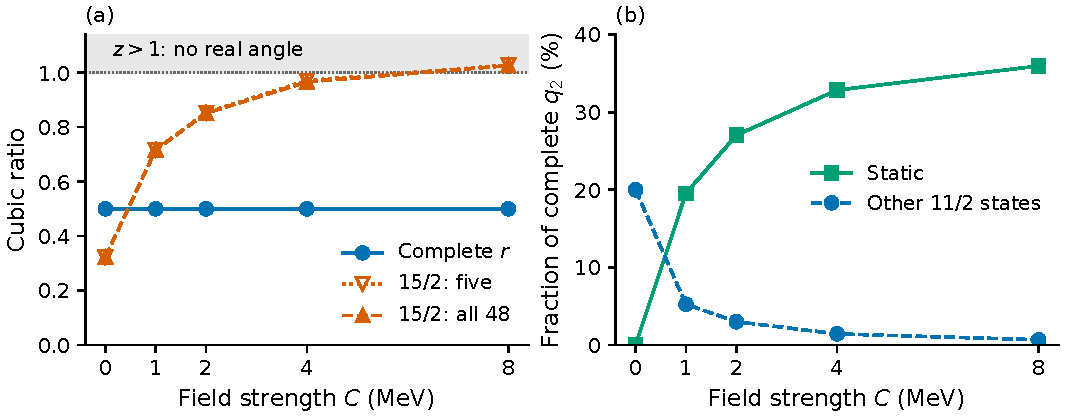
\includegraphics[width=\textwidth]{figures/rigid_charge_control-v1.pdf}
\caption{Independent rigid-charge particle--rotor control at
$\gamma=20^\circ$. (a) Complete ratio and selected-channel ratios using
five or all 48 $15/2$ states. (b) Static and other-same-spin fractions of
$q_2$. The intrinsic tensor and inertias remain fixed at every point;
$C$ has the normalization of Appendix~\ref{app:rigid}.
The shaded region marks the absence of a real selected angle.
Lines join the five calculated points and do not assert untested
continuous-parameter behavior.}\label{fig:rigid}
\end{figure*}

The charge identities were checked as matrices on the entire initial
$11/2$ space, with maximum residual $5.6\times10^{-16}$, and against
independent Euler-angle integration of tensor elements.
All required intermediate spins for its quadratic and cubic closure
are present. Numerical branch matching retains the lowest $11/2$
state in both directions, with minimum adjacent squared overlap 0.648.
The exact geometric identity does not depend on extrapolating that
sampled tracking into a continuous no-crossing claim.


\subsection{Channel saturation and total charge strength}

We next examine the same diagnostic in the IBFM family, which does not impose the rigid-charge operator identities. Table~\ref{tab:results} shows that complete charge strength decreases across the chain, from $q_2=1.53187$ in $^{129}$Ba to $0.47677\,e^2{\rm b}^2$ in $^{137}$Ba. The ratio is $0.3112$. The comparatively weak evolution of the complete normalized cubic moment therefore cannot be interpreted as constant collectivity.



The first five $15/2^-$ states contain $99.59$--$99.85\%$ of the quadratic strength within that spin, but only $20.00$--$28.90\%$ of complete $q_2$ (Table~\ref{tab:results}). Explicit evaluation with every $15/2^-$ state changes the cubic ratio by $|z_5-z_\infty|<0.0093$. For the small $^{129}$Ba ratio this is a $10.7\%$ deviation relative to $z_\infty$, despite an angle shift of only $0.0715^\circ$. In the four cases with a real selected angle, its change is at most $0.259^\circ$. These raw comparisons test cubic convergence directly instead of inferring it from quadratic saturation.

\begin{table}[t]
\caption{Primary model results. $q_2$ is in $e^2{\rm b}^2$; fractions are defined in Eq.~(\ref{eq:fractions}). The signed $r$ and absolute-chain $z_\infty$ use different contractions. $z_\infty>1$ has no real selected angle.}\label{tab:results}
\centering
\setlength{\tabcolsep}{3pt}
\begin{tabular}{crrrrr}
\toprule
$A$ & $q_2$ & $100c_5$ & $100f_5$ & $r$ & $z_\infty$\\
\midrule
129&1.53187&99.62&28.90&$+0.0055$&0.0351\\
131&1.26392&99.59&27.56&$-0.0700$&0.1334\\
133&0.94637&99.84&24.31&$-0.1447$&0.6369\\
135&0.67662&99.85&20.00&$-0.0505$&1.0241\\
137&0.47677&99.62&21.50&$-0.0667$&0.7382\\
\bottomrule
\end{tabular}
\end{table}

The largest qualitative separation occurs in $^{135}$Ba. Its complete signed ratio is $-0.05052$, whereas $z_5=1.02611$. Including the entire selected channel yields $z_\infty=1.02414$, so its failure to define a real angle persists after within-channel completion. In the same state with only the core part of the charge operator, the five-state angle is $3.749^\circ$ and the complete folded angle is $28.561^\circ$. The fermion term changes an already near-boundary selected coordinate into an out-of-domain ratio. The central distinction is therefore visible before the domain crossing; it does not depend on interpreting the crossing as a physical instability.

\subsection{Static strength and signed cubic cancellation}

The quadratic decomposition in Fig.~\ref{fig:channels}(a) reveals a large change in the same-spin sector. In $^{135}$Ba, the static diagonal term carries $33.69\%$ of complete $q_2$, and transitions to other $11/2^-$ states carry another $3.74\%$. The corresponding static fractions in $^{129}$Ba and $^{131}$Ba are only $0.287\%$ and $0.264\%$. Thus the enhanced same-spin strength is primarily static in the $^{135}$Ba case, while the same-spin channel in the lighter pair is dominated by transitions to other states. A description based solely on the selected $15/2^-$ strength does not retain this redistribution.

\begin{figure*}[t]
\centering
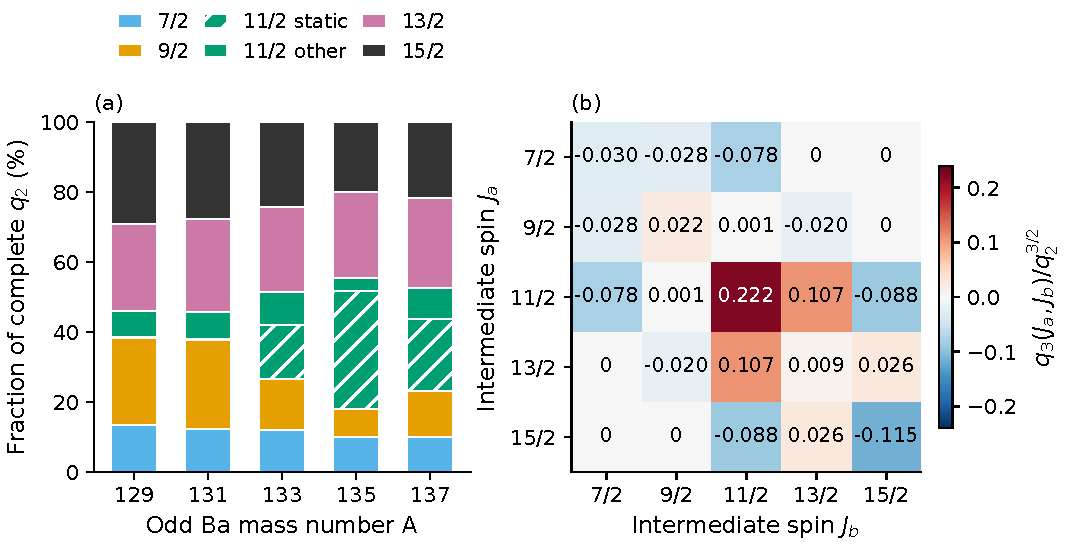
\includegraphics[width=\textwidth]{figures/angular_channels-v4.pdf}
\caption{Decomposition of complete charge moments. (a) Contributions to $q_2$ by intermediate spin. The hatched $11/2$ segment is the static matrix element; the solid segment contains other states of the same spin. (b) Signed contributions to $q_3/q_2^{3/2}$ in $^{135}$Ba, grouped by the ordered pair of intermediate spins. Both matrix orientations are retained in the total sum. Exact angular-momentum selection zeros are shown as zero; other labels are rounded for display.}\label{fig:channels}
\end{figure*}

The complete cubic moment is small because substantial positive and negative contributions cancel. For $^{135}$Ba, their spin-sector sums are $+0.29086$ and $-0.31897\,e^3{\rm b}^3$, respectively, giving $q_3=-0.02812\,e^3{\rm b}^3$. The $15/2$--$15/2$ sector alone contributes $-0.06382\,e^3{\rm b}^3$. It is opposed by the $11/2$--$11/2$ sector, $+0.12335\,e^3{\rm b}^3$, and by both $11/2$--$13/2$ sectors, whose combined contribution is $+0.11950\,e^3{\rm b}^3$. Other sectors complete the cancellation shown in Fig.~\ref{fig:channels}(b).

Equation~(\ref{eq:proxy}) retains only the $15/2$--$15/2$ path, with its own normalization and coefficient. Adding more states within that path cannot recover interference with the omitted spins. The different cubic trends thus correspond to different combinations of the same matrix-element network.
On the common denominator $q_2^{3/2}$, the selected spin sector contributes
$-0.11467$ and all remaining sectors contribute $+0.06415$, producing
$r=-0.05052$. This decomposition keeps the normalization fixed when comparing
the retained and omitted paths.

The operator decomposition also matters after this cancellation. In the fixed $^{135}$Ba state, the core-only cubic moment is $-0.03981\,e^3{\rm b}^3$. Terms containing one or more fermion tensors add $+0.01170\,e^3{\rm b}^3$, moving the complete value toward zero. A small fermion contribution to quadratic strength is therefore insufficient grounds to neglect it in a normalized cubic diagnostic.

\subsection{A controlled quadrupole-coupling path}

To isolate a dynamical origin, we varied the $^{135}$Ba quadrupole coupling as
$\Gamma_0=0.6s$ MeV, with $s=0,0.25,0.50,0.75,1$, while keeping the exchange
and monopole strengths, core, occupation and charge operator fixed.
These are interventions in the model, not alternative fits to the nucleus.
Forward and backward maximum-overlap tracking both select the lowest
$11/2$ state throughout the sampled path. Adjacent squared overlaps exceed
0.907, and the smallest sampled gap to the next state of the same spin is
0.481 MeV. Thus no lowest-state switch is observed at this resolution.

Figure~\ref{fig:path} shows a strong redistribution with little change in total
strength. Complete $q_2$ remains between 0.67662 and
$0.69413\,e^2{\rm b}^2$, a range of less than $2.6\%$, and
$\langle n_d\rangle$ stays between 2.324 and 2.354. The static fraction,
however, rises from $0.0091\%$ to $33.69\%$. The core-$R=2$ probability
increases from 0.0151 to 0.4837, while the core-$R=0$ probability falls
from 0.9522 to 0.4886. In this controlled comparison, quadrupole coupling
principally changes angular recoupling and static polarization rather than
the amount of quadratic charge strength.

\begin{figure*}[t]
\centering
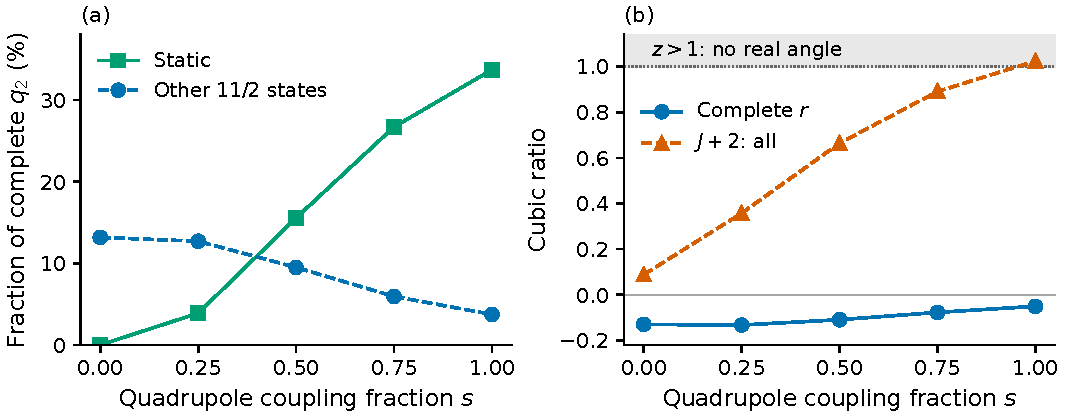
\includegraphics[width=\textwidth]{figures/quadrupole_path-v2.pdf}
\caption{Fixed-exchange/monopole control for $^{135}$Ba:
$\Gamma_0=0.6s$ MeV, $\Lambda_0=1$ MeV, $A_0=-0.9$ MeV.
The core and electric-quadrupole operator are unchanged.
(a) Static and other-same-spin fractions of complete $q_2$.
(b) Complete signed ratio and the all-$15/2$ selected ratio.
Points are the five calculated settings; lines guide the eye.
The shaded region has no real selected angle.}\label{fig:path}
\end{figure*}

The selected ratio rises through a specific change of its numerator and
denominator. Over the path, $S_\infty$ falls from 2.32070 to
$1.62594\,e^2{\rm b}^2$, whereas the signed chain $C_\infty$ grows from
0.37162 to $2.53787\,e^3{\rm b}^3$. In the intermediate energy eigenbasis,
its middle-diagonal contribution changes from
$-0.73467$ to $+1.16709\,e^3{\rm b}^3$: cancellation with off-diagonal
paths is replaced by reinforcement. Consequently $z_\infty$ rises from
0.08795 to 1.02414. At the final point, the additional spin sectors in the
complete cubic moment still largely cancel. Since the all-$15/2$ projector
is unchanged along this path, the result is a change of the initial
state's charge response, not a consequence of reordering a five-state list.

\subsection{Charge-operator and static-moment constraints}\label{sec:emlimits}

The distinction between channel saturation and full coverage survives
35 operator/calibration settings, evaluated on the fixed Ba states:
the primary setting, two fermion charges, two alternative $\chi'$ values
and both quoted-margin core-strength endpoints for each isotope.
Across these settings, the full $15/2$ channel carries 14.12--29.24\%
of $q_2$, and its first five states exhaust 99.588--99.939\% of that channel.
These are deterministic sensitivity tests, not a parameter posterior.

The actual cubic coordinates are more sensitive. In $^{135}$Ba,
$\chi'=0$ or $\chi'=\chi=-0.24$ removes the selected-domain failure and
changes the complete cubic sign. The complete/selected folded angles
become $24.418^\circ/6.241^\circ$ and
$20.166^\circ/10.659^\circ$, respectively. Changing an E2 operator on
one wavefunction is not a change of Hamiltonian shape.

Static moments further constrain nuclear interpretation.
The primary $^{137}$Ba value, $Q_s=+0.77296\,e\,{\rm b}$, agrees with
its source-named calibration target $+0.78(9)\,e\,{\rm b}$ and is not
an independent test. The $^{135}$Ba prediction,
$+1.17693\,e\,{\rm b}$, exceeds the evaluated $+0.96(8)\,e\,{\rm b}$;
Ref.~\cite{Nomura2017} separately quotes $+0.98(8)$ experimentally
and $+1.13\,e\,{\rm b}$ theoretically. The source variants are not averaged.
The primary $^{136}$Ba core moment also disagrees with several evaluated
calibration branches. These discrepancies limit the quantitative static
redistribution that can be assigned to the actual nucleus.

We retained all five finite central-value operator calibrations obtained
from the distinct $^{136}$Ba moment targets, the common core strength
and $Q_s(^{137}{\rm Ba})=0.78\,e\,{\rm b}$, without using $^{135}$Ba to
select a branch. Two branches improve its predicted moment to 0.923 and
$0.915\,e\,{\rm b}$ but give complete ratios $r=-1.093$ and $-1.096$.
Thus even complete moments need not admit a real rigid-equivalent angle.
Appendix~\ref{app:calibrated} retains every branch, the shared-source
and unknown-covariance limitations, and a marginal truncation case.
Matching $Q_s$ through the coupling instead changes the spectrum
(Appendix~\ref{app:momentmatch}); neither calibration is an independent
validation of the electromagnetic network.


\section{Interpretation and scope}\label{sec:discussion}

The fixed-spin comparison separates two structural questions: how much charge-quadrupole strength a state carries, and how particle--core coupling distributes that strength and its interference paths among angular momenta. A selected-channel diagnostic can be sensitive to the second question even after the first is only partially represented. Its sensitivity is potentially useful. Selected matrix-element ratios can also give deformation estimates consistent with invariant analyses within specified low-lying even-even collective regimes \cite{LawrieOrce2025}. Applying a conversion to a mixed odd-$A$ state requires a corresponding test of its coupling regime and charge response.

Prior work establishes approximations to quadrupole moments \cite{Werner2005,Henderson2020}, coupling-dependent $\Delta J$ indicators in odd nuclei \cite{Nomura2016}, and differences between deformation definitions near $A=130$ \cite{Bally2022}. Microscopic restricted-network studies also show how configuration mixing and coverage affect inferred shapes \cite{Rouoof2025}. The present mechanism test combines a fixed-operator intervention with a geometrically fixed control. The former resolves how static strength and signed paths respond in the declared Ba family; the latter demonstrates that variation of the selected diagnostic does not require a change of intrinsic charge shape. Neither the invariant identities nor the existence of channel dependence is new.

The rigid-charge identity is not a claim that the IBFM wavefunctions have
unchanged geometry. Their finite $s,d\otimes h_{11/2}$ space omits
configurations, and products of its effective tensor need not reproduce
the full nucleus's charge moments. The operator alternatives, static-moment
discrepancy and conditional isomer failure limit empirical interpretation.
Neither a moment angle near $30^\circ$ nor a domain crossing identifies
$\gamma$ softness, rigidity or a collective mode.
Furthermore, the published invariant figures of Ref.~\cite{Nomura2017}
remain unreproduced. A difference is already present for its even-core
$J=0$ case, where the spin restriction cannot explain it.
Our conclusions concern the specified operators and states.

\subsection{Empirical reach of the Ba reconstruction}\label{sec:isomer}

A separate high-spin test limits the spectroscopic application.
The tentative $^{137}$Ba $(19/2^-)$ isomer has a reported
589(20)-ns half-life and $B(E2;19/2\to15/2)=0.46(3)$ W.u.\
for its 120.1-keV decay \cite{Vogt2017PRC95_024316}.
The strength is already corrected for conversion and derives from
the same decay evidence as the lifetime.
For each of the two tested model parents, all energetically open
E2 photon rates give
\begin{equation}
T_{1/2}\leq\frac{\ln2}{\sum_f\lambda_{\gamma,f}(E2)}.
\label{eq:isomerbound}
\end{equation}
Across the primary, core-only and five conditional operators,
the largest upper bound is $2.811\times10^{-4}$ ns.
The unchanged modeled schemes cannot represent the observed isomer
under these state identifications. This bound uses model energies
and amplitudes; additional conversion or other positive rates can
only shorten the lifetime of the same scheme.

An alternate selected branch approaches the observed strength,
but a dominant fast route remains open (Appendix~\ref{app:isomer}).
The source-spectrum comparison contains no $19/2$ state and cannot
certify that mapping or attribute the failure to the original authors.
This test limits the reconstruction's high-spin reach without
directly testing the initial-$11/2$ cubic loop, whose rank-two
intermediate spins end at $15/2$.

An observable consequence can be tested before determining the full cubic
network. Define the static-to-first-transition ratio
\begin{equation}
\begin{aligned}
R_{\rm stat}^{(1)}
&=\frac{D_0}{B(E2;11/2_1^-\to15/2_1^-)},\\
D_0&=\frac5{16\pi}\frac{Q_s^2}{55/91}.
\end{aligned}
\label{eq:staticratio}
\end{equation}
Here $55/91=C(11/2,11/2;2,0\mid11/2,11/2)^2$ and $D_0$ is the
diagonal contribution to $q_2$, not a decay strength.
The primary model predicts $R_{\rm stat}^{(1)}=2.2722$ and 1.3565 for
$^{135,137}$Ba, respectively. For a measured reverse decay,
$B_\uparrow=(16/12)B_\downarrow$.
This first-state ratio differs from a sum over all $15/2$ states;
the first state carries about $74\%$ of that model channel in $^{135}$Ba.
An experimental test requires the corresponding level assignment, static
moment and absolute E2 strength. Combining an experimental numerator with a
model denominator would not produce an experimental ratio.
Signed intermediate-state matrix elements would still be needed to test the
cubic cancellation itself.

The audited records provide candidate $(15/2^-)$ levels at 950.5 keV
in $^{135}$Ba and 2229.8 keV in $^{137}$Ba, with respective 682.3-
and 1568.2-keV connections to the $11/2^-$ isomers
\cite{ENSDF,Vogt2017PRC95_024316}. They do not supply the corresponding
absolute E2 denominators. The upper $^{137}$Ba $19/2$ lifetime used
in the separate check of Sec.~\ref{sec:isomer} cannot replace the
$15/2$ parent lifetime. A determination of this first-transition strength,
together with the static moment, would directly test the predicted
redistribution before attempting the full cubic network.
This limitation concerns the specified source set; the tentative assignments
are retained.

\section{Conclusions}\label{sec:conclusion}

Selected-channel convergence does not establish an intrinsic-shape
interpretation for a mixed odd-$A$ state. In the declared Ba model,
quadrupole coupling redistributes static strength and selected cubic paths
while complete quadratic strength changes little. An independent
rigid-charge rotor demonstrates the same diagnostic sensitivity with
geometry exactly fixed. Static-moment discrepancies, operator alternatives
and the conditional high-spin isomer failure bound the nuclear application.
Reporting raw moments, angular-channel coverage and signed contributions
alongside state-count convergence makes these distinct questions testable.

\appendix
\section{Single-shell interaction and tensor ordering}\label{app:conventions}

With $F^{(k)}=[a_j^\dagger\times\widetilde a_j]^{(k)}$, the interaction
used in the IBFM calculations is
\begin{equation}
\begin{aligned}
H_{BF}={}&\Gamma_{jj} Q_\chi\cdot F^{(2)}
+\Lambda_{jj}^{j} X\\
&-A_0\sqrt{2j+1}\,n_dF^{(0)},\\
X={}&:\!\left[[d^\dagger\times\widetilde a_j]^{(j)}
\times[a_j^\dagger\times\widetilde d]^{(j)}\right]^{(0)}\!:\, .
\end{aligned}
\end{equation}
The tilde conventions are
$\widetilde a_{jm}=(-1)^{j-m}a_{j,-m}$ and
$\widetilde d_\mu=(-1)^{2-\mu}d_{-\mu}$.
The exchange term is explicitly normal ordered, retaining the fermion
interchange sign and omitting contractions.
Since $F^{(0)}=-1/\sqrt{2j+1}$ in the one-fermion space, the last term is
$A_0n_d$. Changing it in a control therefore changes the odd-system
$n_d$ coefficient, even when the bare even-core Hamiltonian is fixed.

Scalar and coupled products follow
\begin{align}
A^{(k)}\cdot B^{(k)}&=\sum_\mu(-1)^\mu A_\mu B_{-\mu},\\
[T\times T]^{(2)}_\nu&=\sum_{\mu\eta}
C(2\mu,2\eta\mid2\nu)T_\mu T_\eta .
\end{align}
Operator order and a common eigenvector phase convention are preserved.
No state-independent magnitudes are substituted for signed closed products.

\section{Static-moment matching along the coupling path}\label{app:momentmatch}

Along the fixed-operator path of Fig.~\ref{fig:path}, matching the preselected
$^{135}$Ba values $Q_s=0.88,0.96,1.04\,e\,{\rm b}$ gives
$\Gamma_0=0.33378,0.37929,0.43683$ MeV.
The roots were fixed using only signed static moments before evaluating
the new scalar diagnostics. The complete folded angles are
$28.050^\circ,28.240^\circ,28.473^\circ$, whereas the selected-all angles
are $14.520^\circ,12.371^\circ,9.647^\circ$.
The separation remains $13.53^\circ$--$18.83^\circ$, with both angles real.
All four points, including the separately retained paper-quoted
$Q_s=0.98\,e\,{\rm b}$ alternative, pass direct/reduced closure and
bidirectional matching to the neighboring sampled states.

This is conditional calibration, not an independent validation or a
simultaneous spectroscopic fit. The central match moves the calculated
$15/2_1^--11/2_1^-$ spacing from 691.9 to 526.6 keV, while the tentative
experimental connection is 682.3 keV. For the central $Q_s=0.96\,e\,{\rm b}$
match, the largest absolute change in the first two
states of each spin from $7/2$ to $19/2$, referenced to the corresponding
lowest $11/2$ state, is 0.3684 MeV.
Across all four matched points, that maximum is 0.4322 MeV, at the
$Q_s=0.88\,e\,{\rm b}$ target.
The static moment has been consumed as a calibration input and its
agreement cannot be counted again as independent evidence.

\section{Rigid-charge particle--rotor control}\label{app:rigid}

Using standard particle--rotor kinematics \cite{BohrMottelson1975},
we assemble the unpaired Hamiltonian directly:
\begin{align}
H(C)&=\sum_{k=1}^3 A_k R_k^2+C\,1\otimes Q_j(\gamma),\\
R_k&=I_{k,\mathrm{right}}\otimes1-1\otimes j_k,\nonumber\\
A_k&=\frac{\hbar^2}{2\mathcal J_k},\quad
\mathcal J_k=\frac43\mathcal J_0\sin^2(\gamma-2\pi k/3).
\end{align}
\begin{equation}
\begin{aligned}
Q_j(\gamma)={}&\frac{\cos\gamma}{4j(j+1)}[3j_z^2-j(j+1)1]\\
&+\frac{\sqrt3\sin\gamma}{4j(j+1)}(j_x^2-j_y^2).
\end{aligned}
\end{equation}
The angular momentum components are dimensionless, in units of $\hbar$;
$\mathcal J_0=30\,\hbar^2/{\rm MeV}$, $j=11/2$ and
$\gamma=20^\circ$. The unsorted principal inertias are
38.79385, 16.52704 and $4.67911\,\hbar^2/{\rm MeV}$.
The field $Q_j$ is dimensionless; its normalization defines $C$ and
is distinct from the core-only electric tensor.
There is no pairing projection or zero-gap approximation.

The right-body representation is
$I_{\rm right}=(J_x,-J_y,J_z)$, with
$[I_1,I_2]=-iI_3$; the particle matrices have ordinary commutators.
The full physical $D_2$ subspace is retained at each
$I=1/2,\ldots,15/2$. These 216 multiplets exhaust all required
$7/2$--$15/2$ intermediate states for initial $I=11/2$ quadratic
and cubic closure. They are not a globally complete infinite-rotor space:
for an initial $I=15/2$, additional $17/2$ and $19/2$ channels would be required.

Equation~(\ref{eq:rigididentity}) follows from rotation invariance of
the intrinsic tensor polynomials. Equivalently, its real traceless
Cartesian tensor has
$\operatorname{tr}A^2=1$ and
$\sqrt6\,\operatorname{tr}A^3=\cos3\gamma$ for $\mathcal Q=1$.
The numerical contractions equal these constants times the identity
on the 36-dimensional initial-$I=11/2,M=1/2$ coordinate space.
Independent Euler-angle integration agrees with the product-basis
matrix elements within $2.8\times10^{-14}$.
The independent $D_2$ group projector, tensor covariance and Hermiticity
are checked as well.

At $C=0$, the exact $R_{\rm core}=0$ spectator has zero rotational
energy and static moment. Its spin fractions equal
$(2I_f+1)/[5(2j+1)]$. The two core-$R=2$ energies, 0.126795 and
0.473205 MeV, are recovered independently from a five-dimensional
integer-spin rotor. A deliberately incorrect body-axis sign violates
the zero-energy spectator condition, and omission of the $15/2$
outer sector loses $4/15$ of the initial quadratic closure.
These checks test different parts of the construction without fitting
the selected ratio.

For a fixed axial $K=J$ rotor with intrinsic tensor amplitude
$\mathcal Q=T_{20}^{\rm body}$, the complete moments are
$q_2=\mathcal Q^2$ and $q_3=\mathcal Q^3$.
The conventional electric intrinsic quadrupole moment instead satisfies
$\mathcal Q=\sqrt{5/(16\pi)}Q_0$.
This control illustrates the regime dependence of Eq.~(\ref{eq:proxy}):
at $J=11/2$ it gives $10.193^\circ$ despite axial input.
These controls validate the definitions and implementation; they are not new
shape theorems or empirical uncertainty estimates.

\section{Conditional charge calibrations}\label{app:calibrated}

For each distinct central $^{136}$Ba $2_1^+$ moment target, the
boson charge is kept positive and recalibrated to the common
$B_\uparrow=0.407\,e^2{\rm b}^2$. Its moment determines $\chi'$,
and $Q_s(^{137}{\rm Ba})=0.78\,e\,{\rm b}$ then determines $e_F$.
All finite sign-consistent roots are retained; the $^{135}$Ba
moment is not used. Its boson charge matches the unchanged
$^{134}$Ba core strength.

\begin{table}[t]
\caption{All conditional moment-calibration branches at fixed
Hamiltonians. $t_{136}$, $e_F$ and $Q_s(135)$ are in $e\,{\rm b}$.
Ratios refer to the lowest $^{135}$Ba $11/2^-$ state.
Both $|r|>1$ and $z_\infty>1$ imply an undefined real angle.}
\label{tab:calibrated}
\centering
\setlength{\tabcolsep}{3pt}
\begin{tabular}{rrrrrr}
\toprule
$t_{136}$ & $\chi'$ & $e_F$ & $Q_s(135)$ & $r$ & $z_\infty$\\
\midrule
$-0.19$ & 0.982 & 0.199 & 1.089 & $-0.642$ & 1.030\\
$+0.01$ & 1.959 & 0.311 & 0.923 & $-1.093$ & 0.850\\
$+0.02$ & 2.004 & 0.317 & 0.915 & $-1.096$ & 0.840\\
$+0.07$ & 2.222 & 0.344 & 0.873 & $-1.092$ & 0.792\\
$+0.25$ & 2.943 & 0.445 & 0.723 & $-0.920$ & 0.640\\
\bottomrule
\end{tabular}
\end{table}

The independent E2 parameter $\chi'$ is not restricted here by a
customary interval for the Hamiltonian parameter $\chi$.
These are central-value comparisons at a common averaged core
strength: moment and strength branches may covary, and the 135/137Ba
moment evaluations share source lineage. No joint confidence region
or preference for a branch is inferred.

A marginal domain crossing illustrates the separate role of
state-count truncation. For $^{137}$Ba with the
$+0.01\,e\,{\rm b}$ core target, $z_5=1.00027$ but
$z_\infty=0.99484$, so completing that spin channel restores its
real selected angle. The complete ratio remains $r=-1.08957$.
This differs from the primary $^{135}$Ba crossing that persists
after within-spin completion.

\section{Isomer units, mappings and decay completeness}\label{app:isomer}

The experimental parent and daughter are the tentative $(19/2^-)$
2349.9-keV and $(15/2^-)$ 2229.8-keV levels, respectively.
Their common anchor is the 661.7-keV $11/2^-$ isomer.
For every open model branch, the photon rate used is
\begin{equation}
\lambda_{\gamma,f}(E2)=1.2239\times10^{13}
 E_{if}^{5}B(E2;i\to f),
\end{equation}
with energy, strength and rate units MeV, $e^2{\rm b}^2$ and s$^{-1}$.
No unobserved modeled daughter is treated as an experimentally excluded level.

The ordinary downward Weisskopf reference is
\begin{equation}
B_{\rm W}(E2)=\frac1{4\pi}\left(\frac35\right)^2
(1.2A^{1/3})^4\,e^2{\rm fm}^4.
\end{equation}
For $A=137$, it equals $0.00419544833\,e^2{\rm b}^2$.
Thus the reported $0.46(3)$ W.u.\ corresponds to
$(1.930\pm0.126)\times10^{-3}\,e^2{\rm b}^2$,
with only the source's quoted margin converted.
Our downward strength is
$|R_{15/2,19/2}|^2/20$, while the reverse strength is larger
by $20/16$. This is different from the $16/12$ factor in
Eq.~(\ref{eq:staticratio}) and the factor five for a $0\leftrightarrow2$
core transition.

\begin{table}[t]
\caption{All four predeclared state pairs for the primary $^{137}$Ba
operator. Relative energies use the lowest model $11/2$ state as
zero. The experimental candidate energies on the same reference
are 1688.2 and 1568.1 keV, respectively. Model-state ordinals
do not establish experimental identities.}\label{tab:isomerpairs}
\centering
\begin{tabular}{crrr}
\toprule
$19/2_i\to15/2_f$ & $E_i$ (keV) & $E_f$ (keV) & $B_\downarrow$ (W.u.)\\
\midrule
$1\to1$ &2142.484&968.874&22.46885\\
$1\to2$ &2142.484&2094.159&2.17762\\
$2\to1$ &3648.848&968.874&0.05585\\
$2\to2$ &3648.848&2094.159&13.14225\\
\bottomrule
\end{tabular}
\end{table}

All seven operators---the primary, core-only and five conditional
calibrations---were evaluated for every pair.
The energy-distance mapping was fixed before the E2 evaluation.
The nearest of the four pairs is $19/2_1\to15/2_2$, whose parent
and daughter residuals are still +454 and +526 keV. This minimum
distance is not a certified physical correspondence or a statistical
chi-square fit.
The all-open-width test was defined afterward as a separate
follow-up, without refitting either Hamiltonian or operator.
The full package retains 28 strengths, 14 parent/operator sums and
84 open E2 branches.

For the primary operator, the two parent half-life upper bounds
are $2.69817\times10^{-4}$ and $6.02153\times10^{-5}$ ns.
With the conditional $t_{136}=+0.07\,e\,{\rm b}$ operator,
the alternative $1\to2$ strength is 0.42002 W.u.,
outside the quoted interval $[0.43,0.49]$ W.u.
Its modeled photon energy is only 48.325 keV.
The competing $1\to1$ branch has 21.86655 W.u. and accounts for
99.9981\% of that model's E2 photon rate. These are model rate fractions,
not measured total branching probabilities.

No experimental photon energy is substituted into a different
model branch. Missing conversion and non-E2 rates are not assumed
zero to claim a complete lifetime prediction. Their nonnegativity
gives the conditional upper bound in Eq.~(\ref{eq:isomerbound});
it cannot compensate for the fast E2 routes of the unchanged model scheme.


\backmatter
\bmhead{Data and code availability}
The accompanying \texttt{data/} directory contains the selected evaluated core strengths with provenance, fixed Hamiltonian inputs, calculated scalar decompositions and Python code. The additional rigid-charge, isomer and source-spectrum checks are packaged separately in \texttt{data/revision-v2/}; their producers, adaptation boundaries and replay instructions accompany the results. The original 45-file manifest is preserved. The code requires NumPy and SciPy; figure scripts also use Matplotlib. No private experimental data or publisher full-text files are included. A permanent public repository identifier has not yet been assigned.

\bmhead{AI assistance and draft status}
AI assistance was used for literature retrieval, source comparison, algebraic and numerical implementation, verification and manuscript drafting. The calculations and source records are supplied for inspection. Human author information, contributions and final accountability statements remain to be provided; this manuscript has not been submitted.

\bibliography{references}
\end{document}
